\section{Results and Discussion}

After simulating all possible combinations of algorithm, agent policy, and traffic density, the global metrics were collected and are summarized in the table below:

\begin{figure}[H]
    \centering
    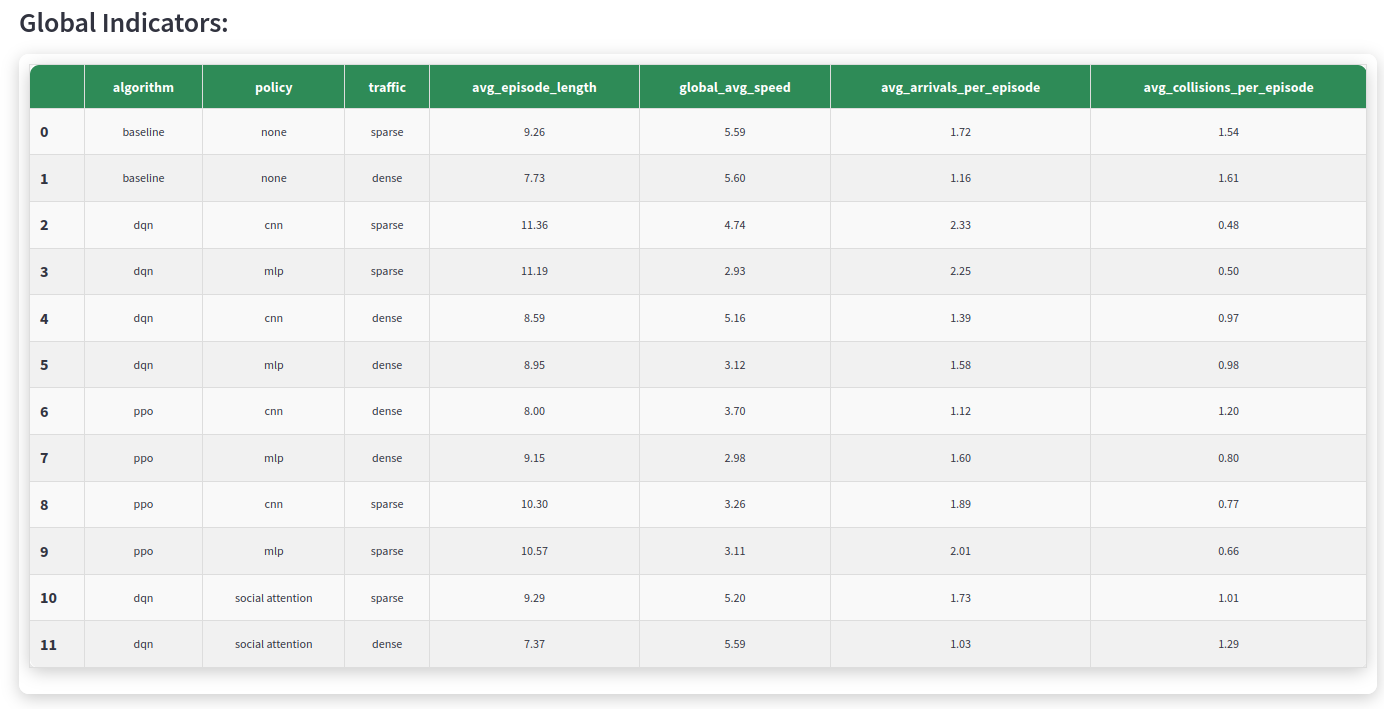
\includegraphics[height=0.42\textheight]{images/app_global_indicators.png} 
    \caption{Summary of Global Metrics for All Algorithm / Policy / Traffic Combinations}
\end{figure}

and plotted:

\begin{figure}[H]
    \centering
    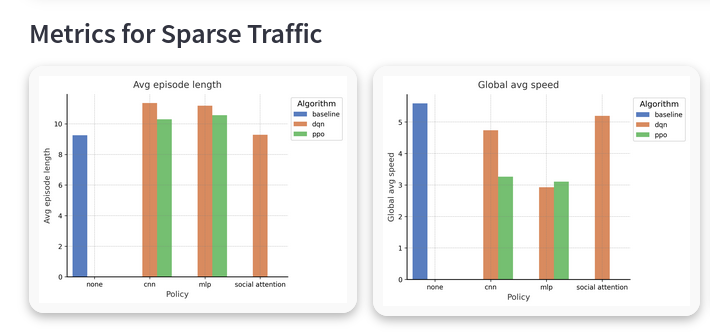
\includegraphics[height=0.22\textheight]{images/app_global_plots_sparse1.png} 
\end{figure}

\begin{figure}[H]
    \centering
    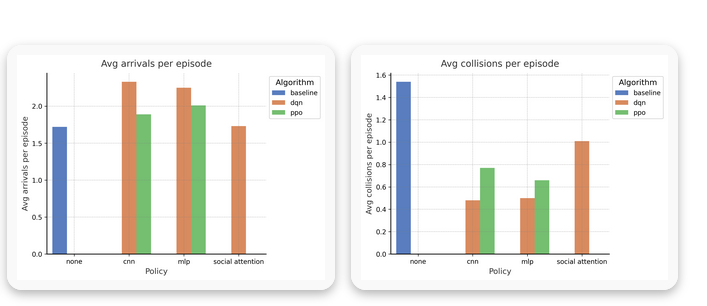
\includegraphics[height=0.19\textheight]{images/app_global_plots_sparse2.png} 
    \caption{Summary of Global Metrics for Sparse Traffic}
\end{figure}

\begin{figure}[H]
    \centering
    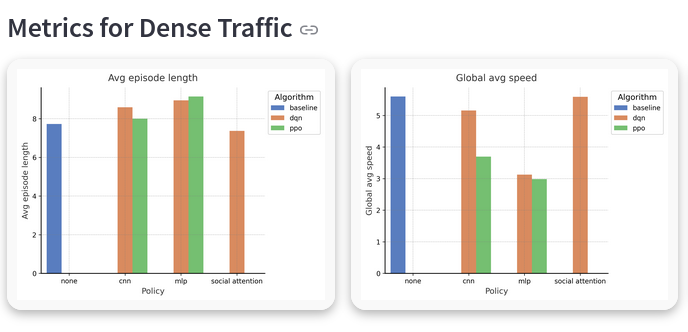
\includegraphics[height=0.215\textheight]{images/app_global_plots_dense1.png} 
\end{figure}

\begin{figure}[H]
    \centering
    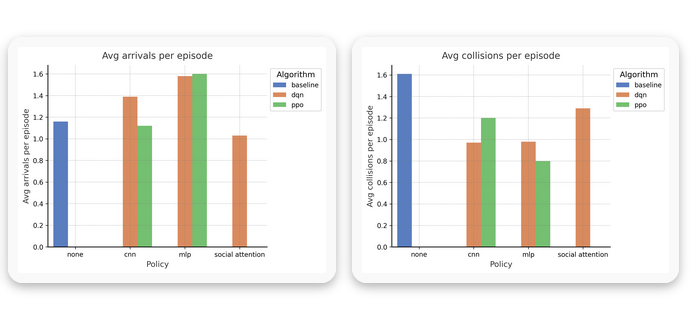
\includegraphics[height=0.2\textheight]{images/app_global_plots_dense2.png} 
    \caption{Summary of Global Metrics for Dense Traffic}
\end{figure}

The results in the table and plots reveal several important trends and insights regarding the performance of the different combinations of algorithm, policy, and traffic density:

\textbf{Average Episode Length}

The average episode length is an important indicator of how well an algorithm handles the traffic conditions without causing early terminations (such as collisions). A longer episode typically suggests that the algorithm is performing well by effectively navigating through the environment, handling traffic without triggering collisions, while shorter episodes may indicate that the agent fails to handle the traffic complexity and encounters more collisions, which results in the early termination of the episode.

In general, the \textbf{average episode length} tends to vary depending on the traffic density, with some algorithms, like PPO, being more resilient in different traffic conditions. These differences in episode length can help evaluate the adaptability of different algorithms to the varying complexities of real-world scenarios, where traffic can range from sparse to dense.
In conclusion, longer episode lengths generally indicate that the algorithms are better at managing traffic randomness and avoiding collisions, leading to smoother, longer episodes. This trend is especially evident in algorithms like DQN, where deeper learning methods tend to produce longer episodes as they allow agents to effectively deal with the traffic complexity. On the other hand, shorter episodes suggest that the algorithm might be struggling with handling the traffic, resulting in earlier episode termination due to collisions.

\textbf{Global Average Speed}

The global reflects the overall efficiency of the agents in the environment. 
It provides an indication of how quickly the agents are able to complete their tasks. 
However, it is essential to consider global average speed in conjunction with other metrics, such as episode length and the number of collisions, 
as a higher speed can sometimes result in more collisions, which would lead to earlier episode terminations.

While higher speeds are generally favorable for achieving higher efficiency, they need to be carefully balanced with the likelihood of collisions and the episode length. 
In this study, the \textbf{baseline} algorithm, which exhibits the highest global speeds, also suffers from shorter episode lengths, suggesting that the increased speed leads to more collisions. 
On the other hand, algorithms like \textbf{dqn} (especially with the \textbf{cnn} and \textbf{mlp} policies) maintain a more balanced speed, leading to longer episodes and fewer collisions. 
This highlights that optimal performance is not solely about speed, but about the balance between speed, collision avoidance, and the ability to handle complex traffic situations.

\textbf{Average Arrivals per Episode and Average Collisions per Episode}

The number of arrivals and collisions are key metrics in assessing the efficiency and safety of the agents' behaviors. 
The total number of arrivals is directly influenced by the number of collisions because the episode ends when a collision occurs, 
which in turn prevents additional arrivals. 
Therefore, these two metrics are inherently linked, with more collisions generally resulting in fewer arrivals.

The number of arrivals is inversely related to the number of collisions, with the highest arrivals typically occurring in configurations that minimize collisions. 
For example, the \textbf{dqn} algorithms, especially with \textbf{cnn} and \textbf{mlp} policies, strike a good balance between speed, collision avoidance, and arrivals, leading to more arrivals due to longer episodes. 
The \textbf{baseline} algorithm, on the other hand, struggles to avoid collisions, leading to fewer arrivals, particularly in dense traffic. 
The \textbf{ppo} algorithm appears less efficient at handling traffic, as evidenced by its higher collision rates, which result in fewer arrivals compared to DQN, particularly in dense traffic.

In essence, the trade-off between arrivals and collisions underscores the importance of careful traffic management and collision avoidance strategies in optimizing the performance of the agents. 
A higher number of arrivals generally indicates a more effective model, as it reflects the agent's ability to avoid collisions and continue the episode until more goals are completed.

Overall, these results highlight the complex interplay between algorithm choice, agent policy, and traffic density in shaping the performance of autonomous driving models. 
The findings also suggest that optimizing for one metric (e.g., speed or arrivals) may negatively impact other factors (e.g., collisions or episode length). 
Further experiments and fine-tuning of algorithms and policies are needed to strike a balance between these competing objectives.

\newpage

\subsection{Performance Indicators and Algorithms Classification}

After calculating the metrics for various algorithms, we can now evaluate the performance indicators and categorize the RL algorithms based on the decision criteria established earlier.

The following results have been derived:

\begin{figure}[H]
    \centering
    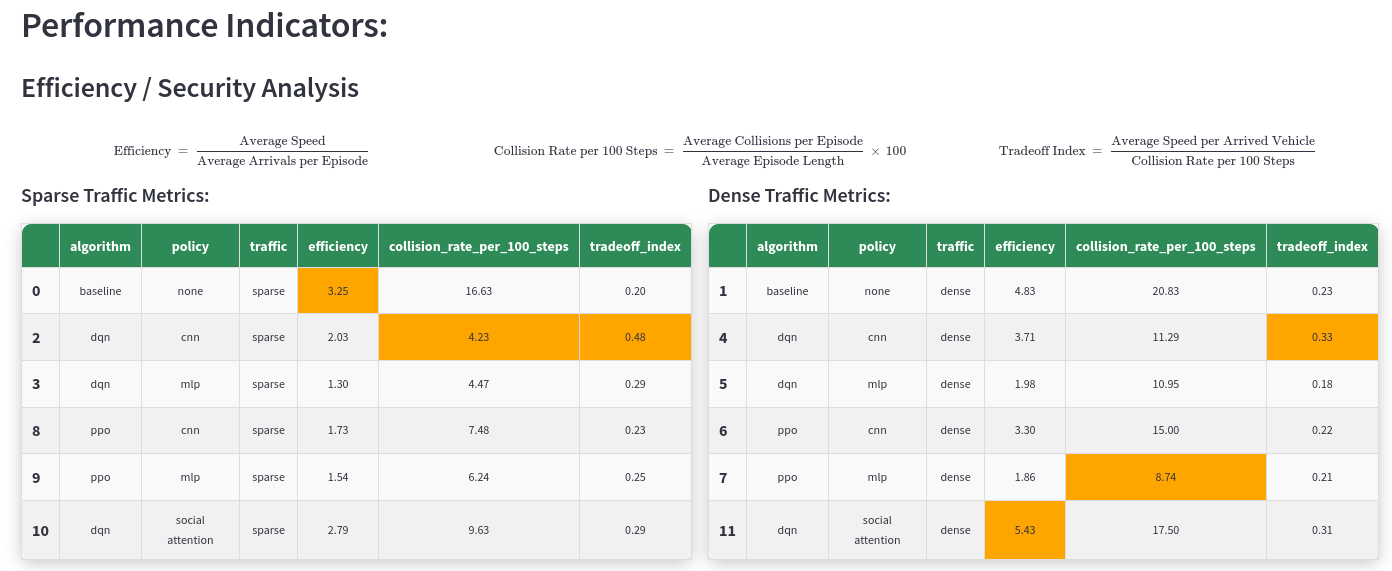
\includegraphics[height=0.3\textheight]{images/app_indicators_efficiency.png} 
    \caption{Efficiency / Security Indicators}
\end{figure}

\textbf{Efficiency/Safety Analysis}

\begin{itemize}
    \item \textbf{Efficiency} is calculated as the ratio of average speed to the average number of arrivals per episode, or inversely, the average arrivals per episode to speed. Higher efficiency values indicate better performance in terms of vehicle throughput.
    \item \textbf{Collision Rate per 100 Steps} is the rate of collisions per 100 steps in the simulation, indicating the safety of the system. A lower rate signifies better safety performance.
    \item \textbf{Tradeoff Index} represents the balance between speed and safety, with a lower value indicating better tradeoff performance (i.e., higher speed with fewer collisions).
\end{itemize}

\textbf{Sparse Traffic Metrics}

In sparse traffic, the baseline algorithm performs the best in terms of efficiency (3.25) but has a relatively high collision rate (16.63). The DQN with CNN policy shows a good balance with an efficiency of 2.03 and a lower collision rate of 4.23, making it a strong performer in sparse traffic. On the other hand, PPO algorithms, particularly with MLP, show lower efficiency and a moderate collision rate.

\textbf{Dense Traffic Metrics}

When traffic density increases, the baseline algorithm maintains its high efficiency (4.83) but faces a significant rise in the collision rate (20.83), reflecting the challenge of maintaining safety in denser traffic. The DQN with social attention policy performs notably well with high efficiency (5.43) and a lower collision rate (17.50) compared to others. In contrast, PPO algorithms continue to show lower efficiency and moderate collision rates, with PPO with MLP showing the lowest tradeoff index.

\begin{itemize}
    \item DQN with social attention seems to strike a good balance between efficiency and safety across both sparse and dense traffic scenarios.
    \item PPO algorithms, particularly with MLP, seem to struggle with efficiency and collision rate tradeoff, particularly in denser traffic.
\end{itemize}


\begin{figure}[H]
    \centering
    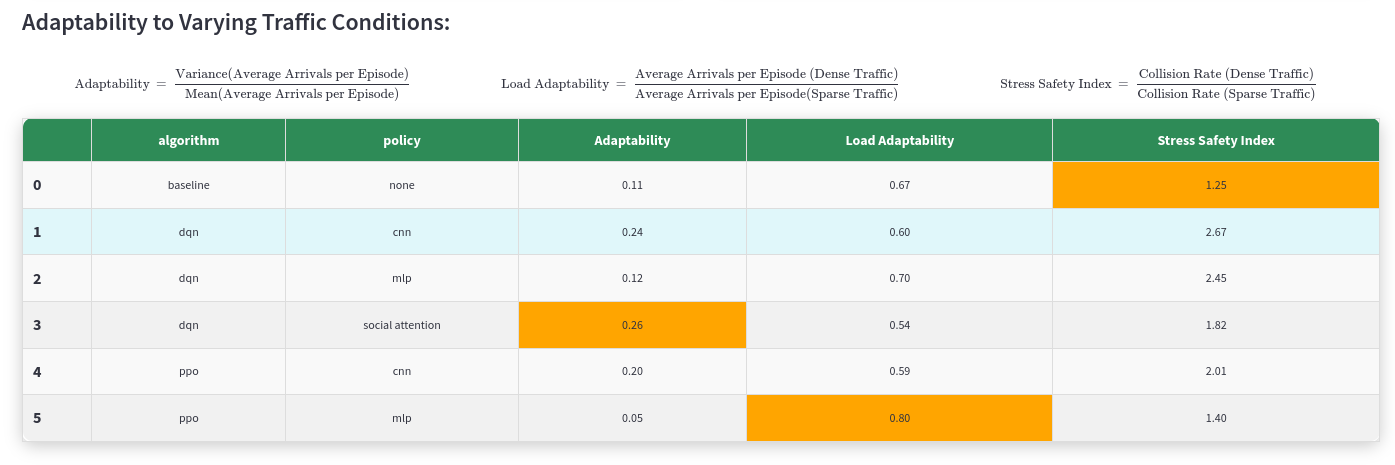
\includegraphics[height=0.25\textheight]{images/app_indicators_adapt.png} 
    \caption{Adaptability Indicators}
\end{figure}

\textbf{Adaptability to Varying Traffic Conditions}

In this analysis, three key metrics are used to assess the adaptability of different algorithms under varying traffic conditions: \textbf{Adaptability}, \textbf{Load Adaptability}, and \textbf{Stress Safety Index}.

\begin{itemize}
    \item \textbf{Adaptability}: This metric measures the variance in the number of arrivals per episode relative to the mean number of arrivals per episode. Higher values indicate better adaptability to changes in traffic conditions. Among the algorithms, the DQN with Social attention policy shows the highest adaptability with a value of 0.26, indicating better ability to adjust to fluctuating traffic conditions. The PPO with MLP policy, on the other hand, shows the lowest adaptability with a value of 0.05.
    
    \item \textbf{Load Adaptability}: This metric compares the algorithm’s performance in dense traffic to sparse traffic. 
    A higher value indicates that the algorithm performs better in dense traffic. The PPO with MLP policy exhibits the highest load adaptability (0.80), showing its ability to handle denser traffic conditions more effectively.
    In contrast, DQN with  Social attention has the lowest load adaptability (0.54), indicating lower performance in dense traffic.

    \item \textbf{Stress Safety Index}: This metric compares collision rates in dense traffic to sparse traffic. 
    A lower value indicates a better safety performance in denser traffic. The PPO with MLP policy shows the best stress safety index (1.40), indicating that it maintains lower collision rates in denser traffic compared to other algorithms. 
    DQN with CNN shows the worst performance in terms of safety, with a stress safety index of 2.67.
\end{itemize}

In summary:

\begin{itemize}
    \item DQN with Social Attention performs well in terms of adaptability, but struggles with load adaptability and stress safety.
    \item PPO with MLP is the best in terms of load adaptability and stress safety, but it has the lowest adaptability.
    \item DQN with CNN shows a balanced performance in all three metrics but does not excel in either adaptability or safety under varying traffic conditions.
\end{itemize}

This allows us to classify the algorithms into High, Medium, and Low categories based on the decision criteria.

\begin{figure}[H]
    \centering
    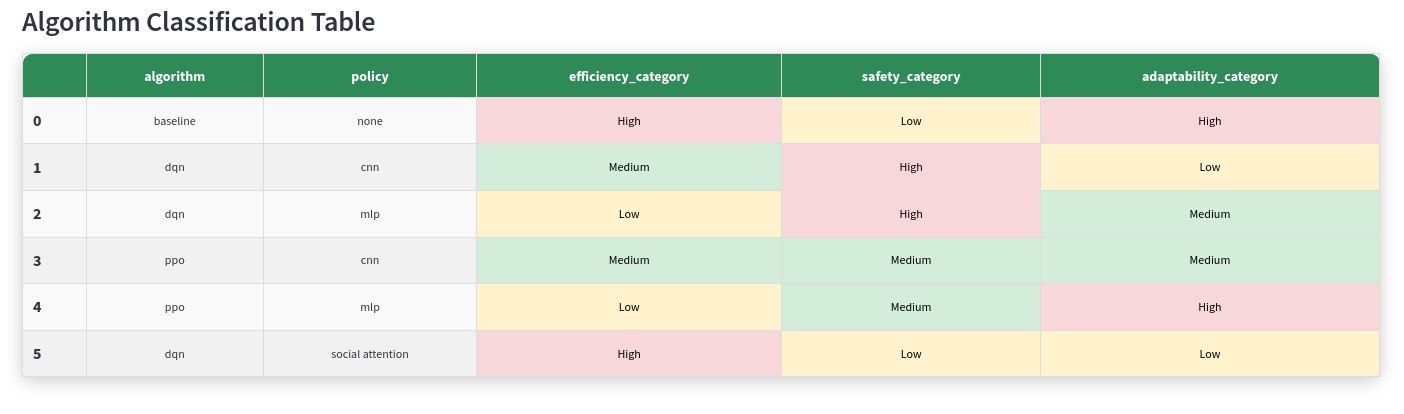
\includegraphics[height=0.22\textheight]{images/app_indicators_classif.png} 
    \caption{Algorithms Classification}
\end{figure}

\textbf{Efficiency:}  
The DQN algorithm with the social attention policy is categorized as \textit{High} in efficiency, indicating its exceptional performance.  
The DQN with CNN and PPO with CNN are classified as \textit{Medium} in efficiency, while the DQN with MLP and PPO with MLP are placed in the \textit{Low} category, reflecting their subpar efficiency.

\textbf{Safety:}  
The DQN with CNN policy excels in safety, earning a \textit{High} classification.  
On the other hand, the DQN with Social Attention and PPO with MLP fall into the \textit{Low} safety category.  
PPO with CNN and DQN with MLP are categorized as \textit{Medium}, indicating an average level of safety.

\textbf{Adaptability:}  
Both the Baseline and PPO with MLP algorithms are classified as \textit{High} in adaptability, showcasing strong performance across varying traffic conditions.  
The DQN with CNN, PPO with CNN, and DQN with MLP are rated as \textit{Medium} in adaptability, while the DQN with Social Attention is ranked \textit{Low} in this metric.

To summarize, The \textbf{DQN} with CNN offers a balanced performance, achieving medium efficiency, high safety, but low adaptability. 
Conversely, the \textbf{PPO} algorithms underperform in both efficiency and adaptability, though they maintain average safety levels. 
Finally, the \textbf{DQN} with Social attention demonstrates good efficiency but is limited by poor adaptability and safety performance.
